\documentclass[12pt,a4paper,twoside]{book}
\usepackage[utf8]{inputenc}
\usepackage{graphicx}
\usepackage{setspace}
\usepackage{emptypage}
\usepackage{geometry}
%\usepackage[showframe]{geometry}
\usepackage{caption}
\usepackage{listings}
\usepackage{color}

\definecolor{code_comment}{RGB}{65,126,96}
\definecolor{code_keyword}{RGB}{126,8,84}
\definecolor{code_string}{RGB}{45,36,251}
\definecolor{gray}{rgb}{0.5,0.5,0.5}

\lstset{
	frame=tb,
	language=Java,
	aboveskip=3mm,
	belowskip=3mm,
	showstringspaces=false,
	columns=flexible,
	basicstyle={\small\ttfamily},
	numbers=left,
	numberstyle=\tiny\color{gray},
	keywordstyle=\color{code_keyword},
	commentstyle=\color{code_comment},
	stringstyle=\color{code_string},
	breaklines=true,
	breakatwhitespace=true
	tabsize=3
}

\DeclareCaptionFormat{listing}{\rule{\dimexpr\textwidth\relax}{0.4pt}\par\addvspace{-6pt} #1#2#3}
\captionsetup[lstlisting]{format=listing,singlelinecheck=false, margin=0pt, font={sf}}

\linespread{1.3}

\begin{document}

	\frontmatter
		\newgeometry{margin=3cm}
\begin{titlepage}
\begin{center}

\begin{large}
	\textbf{POLITECNICO DI MILANO}\\
	Facoltà di Ingegneria\\
	Scuola di Ingegneria dell'Informazione
\end{large}

\vspace{2cm}

\includegraphics[width=3cm]{imgs/poli.eps}

\vspace{2cm}
\begin{large}
\textbf{
DESIGN AND DEVELOPMENT OF AN ASYNCHRONOUS DATA ACCESS LAYER FOR PERVASIVE NETWORKS
}
\end{large}

\vfill

\begin{normalsize}
\begin{onehalfspace}

	\begin{flushleft}
	\begin{tabbing}
	Relatore: \hspace{8pt} \= Ch.mo Prof. Ing. Fabio Alberto Schreiber\\
	Correlatore: \> Ing. Emanuele Panigati
	\end{tabbing}
	\end{flushleft}

	\vspace{1cm}
	\begin{flushright}
	\begin{tabbing}
	\hspace{330pt}
	\= Tesi di laurea di:\\
	\> GUIDO ROTA \\
	\> Matr. 819938\\
	\end{tabbing}
	\end{flushright}
	
\end{onehalfspace}
\end{normalsize}

\vspace{2cm}
\begin{small}
Anno Accademico 2014 - 2015
\end{small}

\end{center}
\end{titlepage}
\restoregeometry

		\include{sommario}
		\chapter*{Sommario}

La presente tesi descrive le fasi di progettazione e sviluppo di un middleware
per la gestione dei dati generati da Sistemi Pervasivi. L'obiettivo principale
di questo software consiste nel fornire un'interfaccia di alto livello
finalizzata all'estrazione di informazioni da un Sistema Pervasivo, vale a dire
una rete eterogenea composta da dispositivi di misura ed attuazione di varia
natura. L'architettura proposta si basa su un paradigma di programmazione ad
eventi che permette una gestione asincrona dei flussi dati generati dalla rete
di sensori controllata.

\chapter*{Abstract}

This thesis describes the design and development of a data management
middleware for Pervasive Systems. The main goal of this software consists in
the definition of a high-level abstraction layer that can be used to collect
information from a Pervasive System, i.e., a heterogeneous network composed of
sensing and actuating devices with different characteristics. The proposed
architecture is based upon an event-driven programming paradigm, which enables
an asynchronous management of the data streams generated by the underlying
sensing network.


		\tableofcontents
		
	\mainmatter
		\chapter{Introduction}

Computing devices permeate every aspect of our life. PCs, tablets, smartphones,
identification badges, credit cards, smart-watches, wearable gadgets, traffic
cameras, digital fitness bands, and personal medical devices like pacemakers or
insulin injectors are only a few of the tools that we use every day, more or
less consciously, to produce and consume information.

As the number of devices and services that surround ourselves increases, so
does the level of mutual cooperation that we expect from them. We know that our
smartphone will automatically show us the weather for our current location,
sometimes even for our hometown when we are away (How does it know where I
live? Did I ever tell it?). Navigation apps guide us through different
itineraries at different times of the day, depending on current and expected
traffic conditions. Outbreaks of the most common viral diseases can be traced
and monitored by analysing what people are searching on the web and correlating
that data with other sources like hospital records.

We have grown so accustomed to the tight level of integration between different
services and information sources, that behaviours similar to those presented
above are nowadays expected. User requirements have heightened, and products
can fail to gain traction if they don’t exploit the data that is available
around us in new and innovative ways; different computing devices and services
must discover themselves and make mutual use of the information that they
produce or consume, meshing together in what is called a Pervasive System.

Firstly envisioned by Mark Weiser [], Pervasive Systems are connected networks
of independent and heterogeneous devices, whose ultimate goal is to assist
people in a way that is effectively invisible to the final user. They are the
result of a post-pc era, where scores of computing gadgets are disseminated in
our surroundings, enhancing our capabilities to sense the world and providing
ubiquitous access to information.

From a software and hardware perspective, a Pervasive Systems is a rich and
varied environment, hosting myriads of different network protocols, data
formats, and incompatible cpu architectures. Tapping the ever increasing stream
of data produced in such a heterogeneous context, and using it to build
advanced and connected products, can easily become a daunting task. Since
Weiser’s seminal paper, several endeavours have explored different techniques
for simplifying the task of building and designing Pervasive Systems, many of
    which stemmed from the research on Wireless Sensor Networks (WSN).

\section{Wireless Sensor Networks and beyond} As suggested by the name,
Wireless Sensor Networks (WSNs) are networks of wirelessly connected devices
called nodes or motes, that are able to measure or detect physical properties
from their surrounding environment. Although the original acronym only
references the sensory features of such systems, current usage of the term WSN
is commonly extended to include devices with actuation capabilities.

Wireless Sensor Networks provide a low-cost and effective solution for
monitoring physical phenomena: several inexpensive nodes may be scattered
around the area of observation, without requiring an explicit configuration or
a wired communication infrastructure. Data is autonomously routed from the
point of origin to the interested consumers, where it is usually aggregated,
analysed and presented to the user. Flexibility and ease of deployment make
WSNs the ideal candidate for a plethora of applications, covering home
automation, theft prevention systems, healthcare, control of environmental
hazards and monitoring of production lines.

The rapid increase in popularity of WSNs, coupled with the intrinsic
difficulties of working with several computing 



\chapter{Data management in Pervasive Systems}

Stato dell'arte, riprenderlo dalla TSE

		\chapter{The PerLa System}

\section{A brief history of PerLa}

\section{Classic middleware architecture}

\subsection{The PerLa query language}

\subsection{Managing heterogeneity: The FPC interface}

What's the FPC, device attributes

\subsection{Network stack}

\subsection{Encoding and decoding data}

\subsection{Interconnecting software components}

\subsection{Device Descriptor and FPC Factory}

Runtime heterogeneity support

\section{Context management}


		\chapter{New middleware architecture}

\section{Design goals and core concepts}

\section{Architecture overview}

The PerLa Middleware is responsible for managing the lifecycle of all devices
connected to the PerLa framework, and for providing a uniform API to interact
with them. Its design revolves around the Functionality Proxy Component
(\texttt{FPC}), a self-contained proxy object that embeds all the logic
required to communicate with a single remote device.  The most prominent trait
of the \texttt{FPC} is its interface, an API that allows PerLa users to
interact with the sensing network through two hardware-agnostic communication
primitives, named get() and set().  Use of this interface neither requires
knowledge of the sensing network, nor of the device that will ultimately
perform the requested operation.

\begin{figure}[h!]
\center
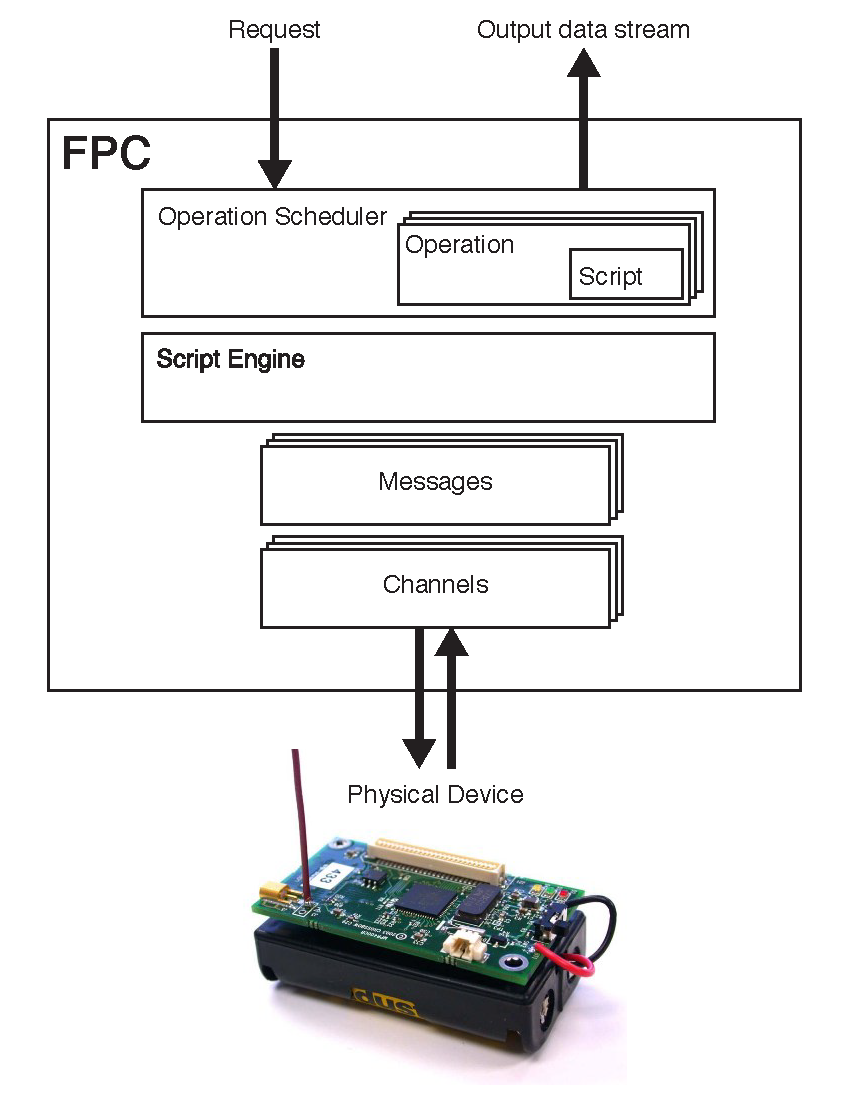
\includegraphics[width=0.6\textwidth]{imgs/fpc.pdf}
\caption{Internal FPC structure}
\label{fig:fpc_overview}
\end{figure}

Each \texttt{FPC} is formed from the composition of various independent
software units, each of which is responsible for the management of a single
aspect of the interaction with the remote device (see
figure~\ref{fig:fpc_overview}). This modular design was chosen to promote
reusability and foster future expandability through composition of
independent objects. The following list contains a synopsis of the modules
that form an \texttt{FPC}:

\begin{itemize}

    \item \textbf{Channel:} A software component capable of performing I/O
    operations. \texttt{Channels} are responsible for managing the
    communication between the PerLa framework and the remote devices;

    \item \textbf{Mapper:} A data marshaller/unmarshaller. \texttt{Mappers}
    allow the \texttt{FPC} to interpret byte streams received from a Channel,
    and to serialize high-level data structures prior to transmission;

    \item \textbf{Script Engine:} An interpreter for executing PerLa
    \texttt{Scripts}, small programs written in a proprietary PerLa scripting
    language, which are used to dynamically bind high level data requests to
    native processing tasks performed on the remote device;

    \item \textbf{Operation Scheduler:} Schedules the execution of concurrent
    data collection operations on the remote device. The scheduler may simulate
    certain operations if the device connected to the FPC is not able to
    perform them natively (e.g., periodic sampling may be simulated by polling
    the remote device at regular intervals).

\end{itemize}

New \texttt{FPC} objects are instantiated at runtime by the
\texttt{FPCFactory}. The starting point for the creation of an \texttt{FPC} is
the Device Descriptor, an XML document which contains a machine parseable
description of a single sensing device. Device Descriptors are organised in
different sections, each of which defines the configuration of one of the
aforementioned \texttt{FPC} modules. The \texttt{FPCFactory} can receive new
Device Descriptors directly from the node being connected (Plug\&Play
behaviour), or from another entity that acts on behalf of it (off-band
behaviour). The latter approach allows devices which are not capable of
autonomously transmit their Device Descriptor to be registered on the PerLa
Middleware.

\begin{figure}[h!]
\label{fig:fpc_overview}
\includegraphics[width=\textwidth]{imgs/middleware_overview.pdf}
\caption{Internal FPC structure}
\end{figure}

A reference to each \texttt{FPC} is stored in the \texttt{Registry}, a
Middleware component that is responsible for maintaining a complete index of
all devices accessible through the PerLa framework. Thanks to the
\texttt{Registry}, PerLa user can discover sensing nodes through
capability-based queries, and retrieve the \texttt{FPC} objects that can be
used to interact with them.

\subsection{Asynchronous interaction paradigm}
\label{sec:newmiddleware.async}

One of the major differences between the New and Classic Middleware
architectures lies in the paradigm employed to interconnect all internal
modules of the PerLa software infrastructure. The New Middleware design
introduces a fully asynchronous interaction paradigm that deviates profoundly
from the mechanism previously promoted, as it is based on the idea of
thread-less module composition.

Within the previous Middleware architecture, a connection between two different
modules was achieved by means of a decoupling element dubbed \texttt{Pipe}, a
one-way message queue designed to shuttle data elements from a software
component to its intended receiver. This system proved to be crucial in the
first development stages of PerLa, as its generic interface allowed the early
designers to experiment with several competing architectures and component
combinations. However, its flexibility came at a cost, both in terms of
performances and API readability. First of all, each \texttt{Pipe} allocated an
initial memory cache of 10 data elements. Moreover, the receiving end of a
\texttt{Pipe}, namely the \texttt{Waiter}, was required to instantiate a Java
thread dedicated solely to the reception of data messages. The widespread use
of the \texttt{Pipe}-\texttt{Waiter} paradigm thus led to the proliferation of
threads and to an overuse of memory, which negatively impacted the overall
system efficiency. In addition, the loosely coupled interaction paradigm
promoted by the Classic Middleware resulted in a weak API that lacked semantic
clarity.

The new 

Although this may not seem as an advantage, as long-running operations must be
performed in a thread nonetheless, short activities



\subsection{Factory patterns}
\label{sec:newmiddleware.factory}

\subsection{Device Descriptor and Plugin system}
\label{sec:newmiddleware.descriptor}

		\chapter{Classic middleware architecture}

\section{Overview}

\section{Netowrk stack}

\section{Encoding and decoding data}

\section{Interconnecting software components}

\section{Device Descriptor and FPC Factory}

		\chapter{New middleware architecture}

\section{Design goals and core concepts}

\section{Architecture overview}

\subsection{Asynchronous invocation paradigm}
\label{sec:newmiddleware.async}

\subsection{Factory patterns}

\subsection{Device Descriptor and Plugin system}
		\chapter{In-depth component description}

\section{Communicating with Channels}

\texttt{Channel} is an interface for performing I/O operations. It represents
the principal abstraction used by the middleware to communicate with hardware
devices and external software services.

\lstset{language=Java}
\begin{lstlisting}[float,caption=The Channel interface,label={lst:channel}]
public interface Channel {

	public String getId();
	
	public IOTask submit(IORequest request, IOHandler handler)
			throws ChannelException;
	
	public void setAsyncIOHandler(IOHandler handler)
			throws IllegalStateException;
			
	public boolean isClosed();
	
	public void close();
			
}
\end{lstlisting}

The \texttt{Channel} interface is not tied to any specific technology or
communication stack; as a result of this design choice, a wide variety of data
management tasks, including but not limited to, networking, file handling, and
automatic data generation can be implemented as \texttt{Channel}s.

The current middleware architecture encourages the creation of several highly
specialized \texttt{Channel}s, which are usually developed around third-party
communication libraries. \texttt{HTTPChannel}, a \texttt{Channel} providing
support for HTTP communications, is an excellent example of the advantages of
this design strategy. Implemented as a simple wrapper around Apache's HTTP
Components toolkit, its development only required a basic understanding of the
HTTP protocol; yet \texttt{HTTPChannel} is a fully compliant HTTP/1.1 client
(see section~\ref{sec:channel.implementations} for additional details).

Upon instantiation, \texttt{Channel}s are open and ready to be used. They may
be optionally closed to relinquish unused resources by invoking the
\texttt{close()} method. Once closed, a \texttt{Channel} cannot be re-opened,
and every subsequent attempt to perform an I/O operation will fail causing a
\texttt{ChannelException} to be thrown. The current state of a \texttt{Channel}
can be probed through its \texttt{isClosed()} method.

Bytes sent or received with a \texttt{Channel} are encapsulated within a
\texttt{Payload}, an object whose interface (listing~\ref{lst:payload}) allows
\texttt{Channel}s and other data manipulation components to handle different
data types regardless of the particular data representation chosen by the
Middleware. \texttt{Payload}s will be the subject of further discussion in
section~\ref{sec:components.mapper}

\lstset{language=Java}
\begin{lstlisting}[float,caption=The Payload interface,label={lst:payload}]
public interface Payload {

	public Charset getCharset();

	public InputStream asInputStream();

	public ByteBuffer asByteBuffer();

	public String asString();

}
\end{lstlisting}

All user-initiated I/O operations begin with an invocation of the
\texttt{Channel.submit()} method. As can be seen in listing~\ref{lst:channel},
\texttt{submit()} is a direct implementation of the asynchronous interaction
paradigm introduced in section~\ref{sec:newmiddleware.async}. The emphasis on
asynchronous execution is underscored by the absence of blocking operations in
the \texttt{Channel} interface. This aspect is of paramount importance for the
entire Middleware design, as implementing a truly asynchronous system would
prove impossible if such feature were not provided by its core data access
layer.


\section{Instantiating new Channels}

Creation of new \texttt{Channel}s is performed by means of the
\texttt{ChannelFactory} interface, a reification of the Factory design pattern
that allows polymorphic instantiation of object classes.

By using the Factory instantiation model, the choice of a particular
\texttt{Channel} implementation can be postponed from compile time to run time.
This technique allows the Middleware to dynamically adapt in response to
environment changes, and to support extension through the addition of new
user-defined \texttt{Channel}s. For further information regarding the Factory
pattern and its uses inside the PerLa Middleware, refer to
section~\ref{sec:newmiddleware.factory}.

All the information required to create a new \texttt{Channel} is stored inside
a \texttt{ChannelDescriptor}. As shown in listing~\ref{lst:channelFactory},
this configuration object is the only parameter required to correctly invoke
the \texttt{createChannel()} method.

\lstset{language=Java}
\begin{lstlisting}[float,caption=The ChannelFactory
interface,label={lst:channelFactory}]
public interface ChannelFactory {

	public Class<? extends ChannelDescriptor>
			acceptedChannelDescriptorClass();

	public Channel createChannel(ChannelDescriptor descriptor)
			throws InvalidDeviceDescriptorException;

}
\end{lstlisting}

\begin{figure}[h!]
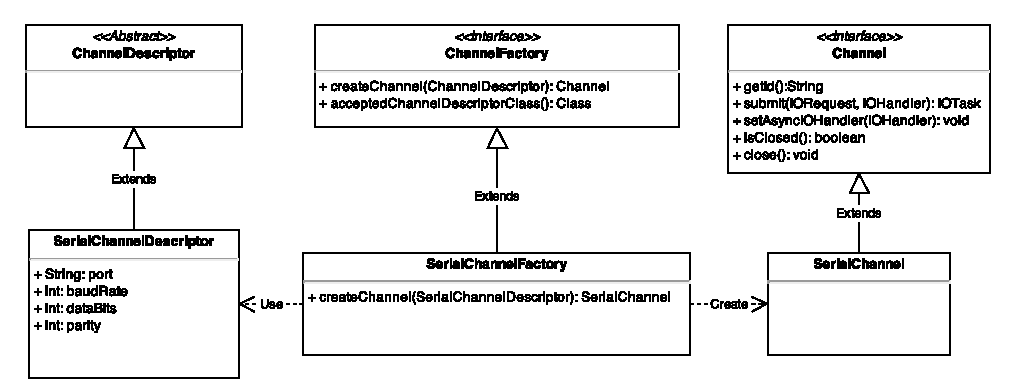
\includegraphics[width=\textwidth]{imgs/channel_factory.pdf}
\caption{Class diagram of the Channel layer}
\end{figure}

Each \texttt{ChannelFactory} is tied to a specific communication technology;
therefore, it can only accept a single class of \texttt{ChannelDescriptor}
objects. For example, the \texttt{HTTPChannelFactory} parses
\texttt{HTTPChannelDescriptor}s and creates \texttt{HTTPChannel}s, whereas an
hypothetical \texttt{SerialChannelFactory} would consume
\texttt{SerialChannelDescriptor}s to create \texttt{SerialChannel}s. Failure to
provide a suitable \texttt{ChannelDescriptor} object will cause the
\texttt{createChannel()} method to throw an
\texttt{InvalidDeviceDescriptorException}.

The \texttt{acceptedChannelDescriptorClass()} method can be used to dynamically
discover which \texttt{ChannelDescriptor} type is supported by a specific
\texttt{ChannelFactory}. This method is the fulcrum of the \texttt{Channel}
Plugin System, as it allows the Middleware to invoke the most appropriate
\texttt{ChannelFactory} using only information available at runtime.

\begin{figure}[!hbt]
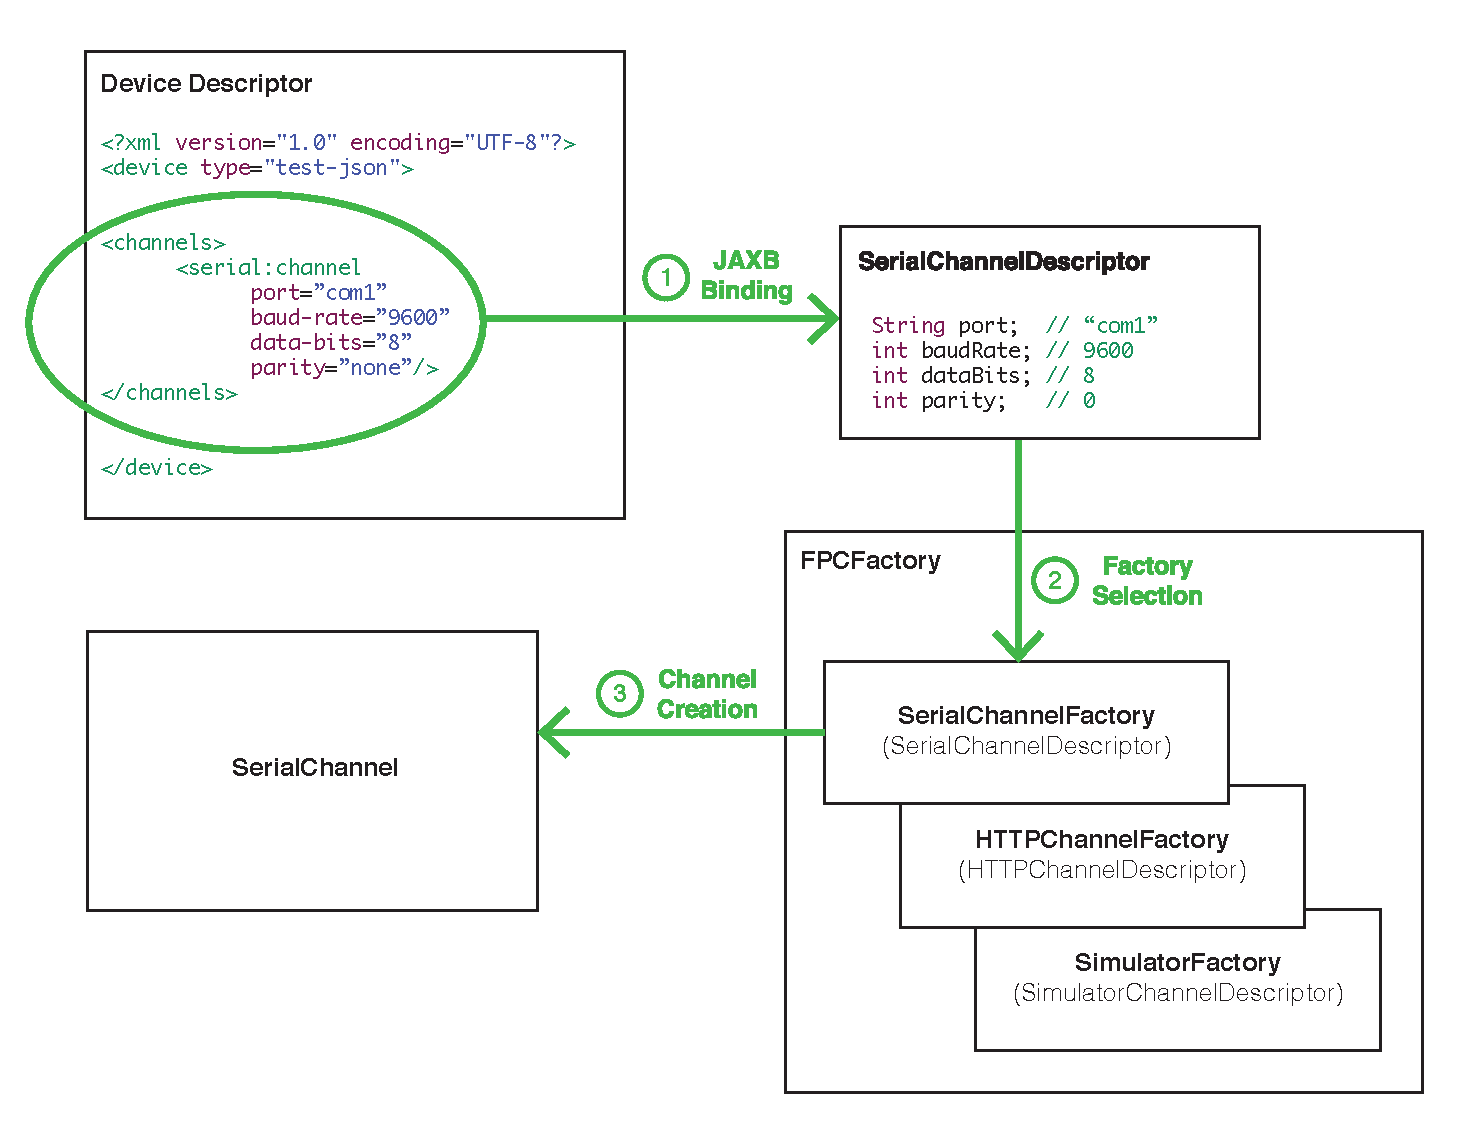
\includegraphics[width=\textwidth]{imgs/channel_creation_process.pdf}
\caption{The Channel creation process}
\label{fig:channel.creation}
{
\begin{figurenote}
This figure illustrates the \texttt{Channel} creation process executed by the
Middleware upon reception of a new Device Descriptor.  \begin{enumerate}
  \itemsep0em
  \item JAXB binds the XML Device Descriptor to an apropriate
\texttt{ChannelDescriptor} object using namespace information \item A suitable
\texttt{ChannelFactory} is selected at runtime using the
\texttt{acceptedChannelDescriptorClass()} method
  \item The information contained in the \texttt{SerialChannelDescriptor} is
used to create a new \texttt{SerialChannel} \end{enumerate}
\end{figurenote}
}
\end{figure}

\texttt{ChannelDescriptor} objects are automatically instantiated by the
Middleware using the information contained in the Device Descriptor XML files.
This binding process is performed by the JAXB library, which is also
responsible for instantiating the correct \texttt{ChannelDescriptor} class
using XML Namespace information. Figure~\ref{fig:channel.creation} illustrates
this technique, and ties it together with the other operations described in
this section.

It is important to note that a single JVM instance running the PerLa Middleware
may host several \texttt{Channel} objects of the same type, at the same time.
Several devices can use the same communication technology, and the
\texttt{ChannelFactory} may determine that it's best to create an individual
\texttt{Channel} for each one of them. This behaviour is fostered by the new
\texttt{ChannelFactory} architecture, and is considered idiomatic design;
hence, it would not be uncommon to implement the hypothetical
\texttt{SerialChannelFactory} introduced in the previous paragraphs so that
every serial port is handled by a different \texttt{SerialChannel} instance.


\subsection{IORequest management}

\texttt{IORequest} is the base object interface employed to interact with a
device connected to the Middleware. It contains two types of information: the
payload to be transferred, and \texttt{Channel}-dependent data needed for a
correct communication with the endpoint device.

\lstset{language=Java}
\begin{lstlisting}[float,floatplacement=!hbt,caption=The IORequest
interface,label={lst:iorequest}]
public interface IORequest {

	public String getId();

	public void setParameter(String name, Payload payload);
	
}
\end{lstlisting}

Since different communication technologies require different configuration
settings to establish end-to-end connectivity, every \texttt{Channel} is
bundled with one or more custom \texttt{IORequest} classes. Following up on
previous examples, the \texttt{HTTPChannel} package contains a
\texttt{HTTPIORequest} object, whereas the fictitious \texttt{SerialChannel}
would be supplied with a \texttt{SerialIORequest} class of request objects.

As shown in listing~\ref{lst:iorequest}, payload data can be set in an
\texttt{IORequest} by means of the \texttt{setParameter()} method.
\texttt{Payload}s are addressed by name, and a single \texttt{IORequest}
implementation may support several at once. The exact set of \texttt{Payload}
parameters accepted by an \texttt{IORequest} class depends on the design of the
associated \texttt{Channel}; for example, the \texttt{HTTPChannel}
implementation provided with the Middleware supports three: an `entity' payload
(request body), a `query' payload (an URL-encoded string), and a `path' payload
(a path component used to identify a single resource accessible from the base
URL).

\texttt{IORequest}s are disposable objects; they are created, submitted to a
\texttt{Channel}, and garbage collected once the communication is over.
Creation is performed by means of a factory interface dubbed
\texttt{IORequestBuilder}, which allows the Middleware to build new copies of
an \texttt{IORequest} from a fixed template. It is important to note that
request objects built using this technique do not contain any \texttt{Payload}
parameter; these are to be added manually before subbmitting the
\texttt{IORequest} to a \texttt{Channel}.

A single device connected to the PerLa Middleware is generally managed using
several \texttt{IORequestBuilder}s, any one of which is responsible for
creating requests that control a single aspect of the interaction with the
endpoint. The main advantage brought by this templating mechanism is that
\texttt{Channel}-related configuration settings are only specified once, hence
the same \texttt{IORequest} structure can be reused multiple times to transport
different payload information.

\lstset{language=Java}
\begin{lstlisting}[float,floatplacement=!hbt,caption=The IORequestBuilder
interface,label={lst:iorequestbuilder}]
public interface IORequestBuilder {

	public String getRequestId();

	public IORequest create();

	public abstract List<IORequestParameter> getParameterList();

	public static class IORequestParameter {

		public String getName() {
			return name;
		}

		public boolean isMandatory() {
			return mandatory;
		}

	}
}
\end{lstlisting}

REST APIs are an excellent use case to demonstrate the aforementioned concept,
as every operation on a RESTful resource can be easily abstracted using an
appropriately configured request builder. By using
\texttt{HTTPIORequestBuilder} objects, HTTP protocol information (base URL,
method, header information, \ldots) are specified one single time only for
every REST endpoint. Once this step is done, the API can be invoked just by
building new \texttt{IORequest}s and submitting them to a \texttt{HTTPChannel}.

Besides \texttt{IORequest} creation, the \texttt{IORequestBuilder} interface
can be used to dynamically discover all \texttt{Payload} parameters supported
by an \texttt{IORequest}. This functionality, exposed through the
\texttt{getParameterList()} method, is a crucial component of the Middleware
Plugin System, as it allows \texttt{Script} instructions to determine whether
an \texttt{IORequest} was correctly populated with all the necessary
\texttt{Payload} parameters or not. This concept will be the subject of further
analysis in section~\ref{sec:components.script}.

\begin{figure}[!hbt]
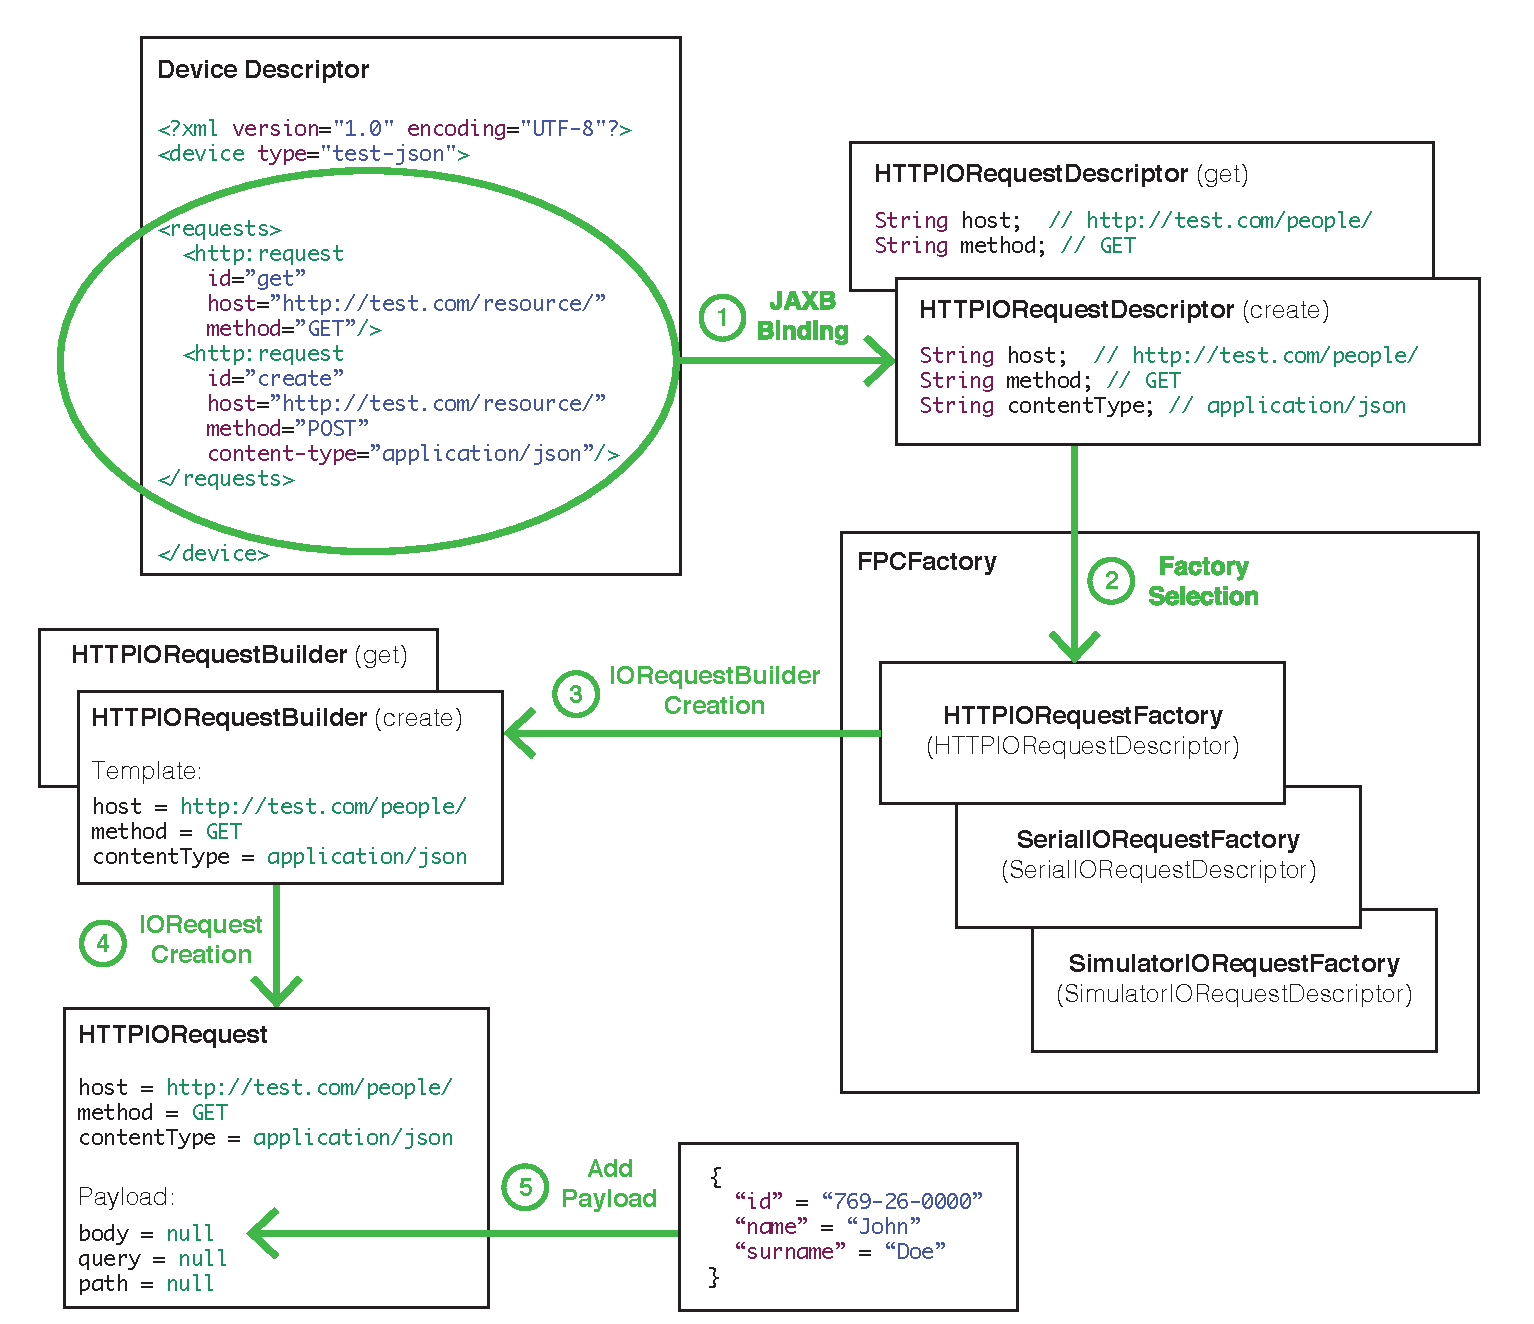
\includegraphics[width=\textwidth]{imgs/iorequest_creation_process.pdf}
\caption{The IORequest creation process}
\label{fig:iorequest.creation}
{
\begin{figurenote}
This figure illustrates the autonomous creation of \texttt{IORequest} objects.
Steps 1 to 3 are performed only once after receiving the Device Descriptor,
whereas steps 4 and 5 are repeated every time the REST API is to be invoked.
\begin{enumerate}
  \itemsep0em
  \item JAXB binds the XML Device Descriptor to an apropriate
\texttt{IORequestDescriptor} object using namespace information \item A
suitable \texttt{IORequestBuilderFactory} is selected at runtime using the
\texttt{acceptedIORequestDescriptorClass()} method
  \item The information contained in the \texttt{IORequestDescriptor} is used
to create a new \texttt{IORequestBuilder} \item The \texttt{IORequestBuilder}
is used to create new \texttt{IORequest} copies using the internal template
  \item The newly created \texttt{IORequest} objects can be populated with
\texttt{Payload} parameters as needed \end{enumerate}
\end{figurenote}
}
\end{figure}

\texttt{IORequestBuilder}s are created by means of an
\texttt{IORequestBuilderFactory}, an object that implements the now familiar
Factory design pattern. Similarly to what already seen in the previous section,
every \texttt{IORequestBuilderFactory} implements an
\texttt{acceptedIORequestDescriptorClass()} method, which can be used to
dynamically determine if a factory object can parse a specific type of
\texttt{IORequestDescriptor}.   It should come as no surprise that every
\texttt{IORequestBuilder} class is provided with complementary
\texttt{IORequestBuilderFactory} and \texttt{IORequestDescriptor}
implementations.

Creation of a new \texttt{IORequestBuilder} object proceeds as follows: The
template for creating new \texttt{IORequest} objects is loaded from an XML
Device Descriptor, bound to an appropriate \texttt{IORequestDescriptor}, and
processed by the \texttt{IORequestBuilderFactory} to create the corresponding
\texttt{IORequestBuilder}. Figure~\ref{fig:iorequest.creation} provides a
comprehensive overview on this process and on the management of
\texttt{IORequest} objects.

\begin{figure}[!hbt]
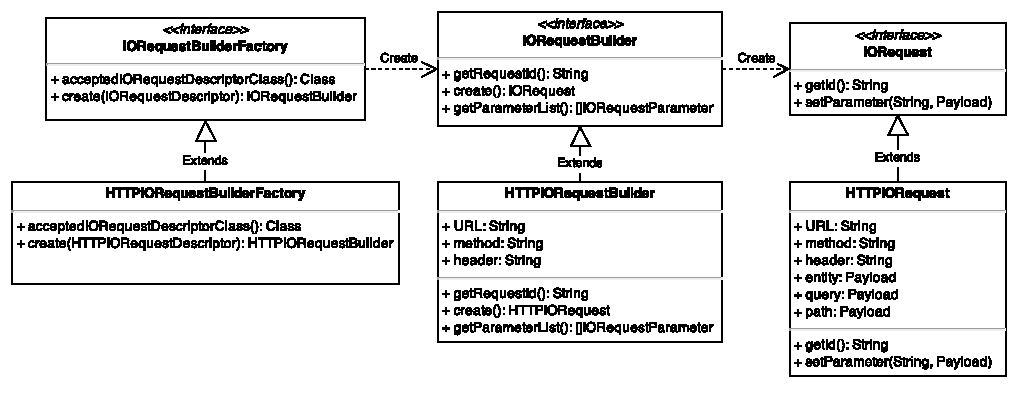
\includegraphics[width=\textwidth]{imgs/iorequest.pdf}
\caption{The extended IORequest class diagram. For additional information about
the IORequestParameter object consult listing 1.5.} \label{fig:iorequest.class}
\end{figure}


\subsection{Handling asynchronous I/O operations}

As mentioned in previous sections, communication with a device connected to the
PerLa Middleware is achieved by means of the \texttt{Channel.submit()} method.
Invocations of \texttt{submit()} are non-blocking; control flow is immediately
returned to the caller, thus allowing other computations to be performed while
the requested I/O operation is being processed.

As can be seen in listing~\ref{lst:channel}, \texttt{submit()} requires two
parameters: an \texttt{IORequest} and an \texttt{IOHandler} callback interface.
The former specifies which I/O operation is to be performed, while the latter
allows the caller to be asynchronously notified of its completion.

The \texttt{IOHandler} interface is composed of a \texttt{complete()} method
and an \texttt{error()} method, which are invoked by the \texttt{Channel} when
the processing of an I/O operation completes or fails respectively. It is
important to note that both these methods always carry context information in
the form of an \texttt{IORequest}, which is guaranteed to be the same exact
object submitted to the \texttt{Channel} when starting the I/O operation whose
completion is being notified. For this reason, \texttt{IOHandler} can be
considered the nexus of the asynchronous invocation model, as it connects
\texttt{IORequest} objects with the outcome of the corresponding I/O operation
performed by the \texttt{Channel}.

\lstset{language=Java}
\begin{lstlisting}[float,floatplacement=H,caption=The IOHandler interface,label={lst:iohandler}]
public interface IOHandler {
	public void complete(IORequest request, Optional<Payload> result);
	
	public void error(IORequest request, Throwable cause);
}
\end{lstlisting}

Semantically, an invocation of the \texttt{complete()} method is always
associated with the successful termination of an I/O operation. As shown in
listing~\ref{lst:iohandler}, this method includes an optional \texttt{Payload}
object that contains all data received from the endpoint device. A call to
\texttt{complete()} with an empty \texttt{Payload} indicates that the I/O
operation was completed without errors, but no data was received. Conversely,
an invocation of the \texttt{error()} method indicates that the I/O operation
was aborted before completion. In this case the cause of failure is always
notified through the \texttt{cause} parameter.

From the point of view the Java memory model, the \texttt{Channel.submit()}
creates a happens-before relationship with \texttt{IOHandler.complete()} and
\texttt{IOHandler.error()}, viz. the effects generated by the code that led to
the \texttt{submit()} invocation are visible from inside the code executed in
the \texttt{complete()} and \texttt{error()} callback methods.

Asynchrous execution does not imply loss of control; ongoing I/O operations can
be monitored or cancelled by means of the \texttt{IOTask} object acquired upon
submitting an \texttt{IORequest}. Listing~\ref{lst:iotask} shows all methods of
the \texttt{IOTask} interface; method names are self explanatory, and the
reader should be able to deduce their purpose just by analyzing the method
signature. The only nuance that is worth mentioning is that
\texttt{isCancelled()} always implies \texttt{isDone()} (i.e., all cancelled
I/O operations are also complete), while the opposite does not hold (i.e., not
all complete I/O operations were cancelled).

\lstset{language=Java}
\begin{lstlisting}[float,floatplacement=!hbt,caption=The IOTask
interface,label={lst:iotask}]
public interface IOTask {
	public void cancel();
	
	public IORequest getRequest();
	
	public boolean isCancelled();
	
	public boolean isDone();
}
\end{lstlisting}

The \texttt{Channel} interface is also designed to manage completely
asynchronous I/O operations, namely communication efforts spontaneously
initiated by the remote device. This communication model is popular among WSNs,
and it is often employed to handle periodic streams of data or events happening
at irregular intervals. Such I/O operations can be handled through a catch-all
\texttt{IOHandler} set with the \texttt{setAsyncIOHandler()}
(listing~\ref{lst:channel}). Since the communication is not initiated by the
Middleware, the \texttt{complete()} and \texttt{error()} callback methods will
be invoked with the \texttt{IORequest} parameter set to \texttt{null}.

\begin{figure}[!hbt]
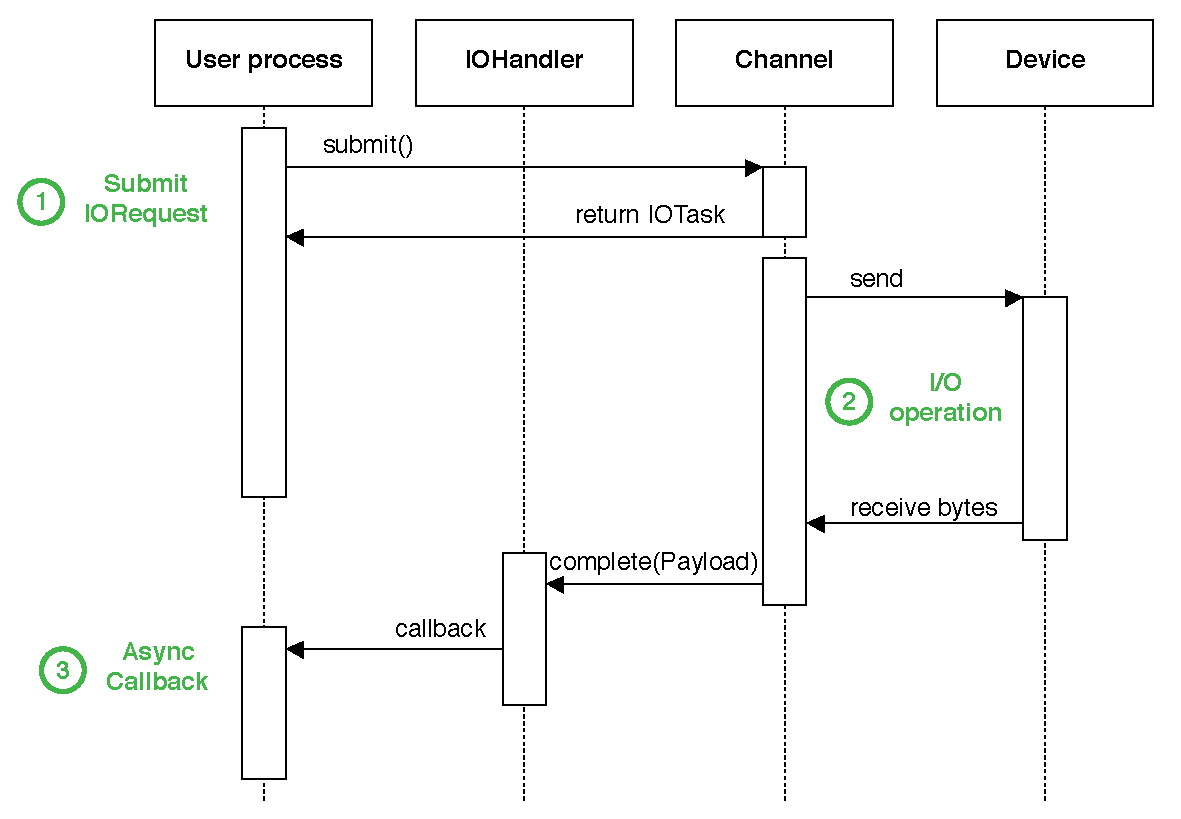
\includegraphics[width=\textwidth]{imgs/async_channel_sequence.pdf}
\caption{Sequence diagram of an asynchronous I/O operation. Note that the user
process and the I/O operation are executed in parallel.}
\label{fig:channel.async}
\end{figure}



\subsection{Implementations: HTTPChannel and SimulatorChannel}
\label{sec:channel.implementations}

Full examples of actual implementations, complete with XML descriptor snippets


\section{Encoding and decoding information}
\label{sec:components.mapper}

\subsection{The Message and Mapper interfaces}

\subsection{Handling composite data structures}

\subsection{Managing multiple message types}

\subsection{Implementations: JSONMapper and URLEncodedMapper}


\section{Data management: Scripts}
\label{sec:components.script}

\subsection{From Messages to Records}

\subsection{Available instructions}

\subsection{Engine architecture and execution model}

\subsection{Script examples}


\section{Putting it all together: the FPC}

\subsection{Data access interface}

\subsection{Controlling the remote device}

\subsection{Scheduling mechanism}


\section{Device Descriptor and FPC Factory}

\subsection{The XML Device Descriptor}

\subsection{FPC Factory}

\subsection{Registry}

\subsection{Complete XML Device Descriptor examples}

		\include{chapter7}

	\appendix


\end{document}
